\chapter{Metrization Theorems and Paracompactness}

The Urysohn metrization theorem of Chapter 4 was the first step-a giant one-toward an answer to the question: When is a topological space metrizable? It gives conditions under which a space \(X\) is metrizable. that it be regular and have a countable basis. But mathematicians are never satisfied with a theorem if there is some hope of proving a stronger one. In the present case, one can hope to strengthen the theorem by finding conditions on \(X\) that are both necessary and sufficient for \(X\) to be metrizable, that is, conditions that are equivalent to metrizability.

We know that the regularity hypothesis in the Urysohn metrization theorem is a necessary one, but the countable basis condition is not. So the obvious thing to do is try to replace the countable basis condition by something weaker. Finding such condition is a delicate task. The condition has to be strong enough to imply metrizability, and yet weak enough that all metrizable spaces satisfy it. In a situation like this, discovering the right hypothesis is more than half the battle.

The condition that was eventually formulated, by J. Nagata and Y. Smurnov independently, involves a new notion, that of local finiteness. We say that a collection \(\mathcal{A}\) of subsets of a space \(X\) is locally finite if every point of \(X\) has a neighborhood that intersects only finitely many elements of \(\mathcal{A}\) .

Now one way of expressing the condition that the basis \(\mathcal{B}\) is countable is to say that \(\mathcal{B}\) can be expressed in the form

\[
\mathcal{B} = \mathop{\bigcup }\limits_{{n \in  {\mathbb{Z}}_{ + }}}{\mathcal{B}}_{n}
\]

where each collection \({\mathcal{B}}_{n}\) is finite. This is an awkward way of saying that \(\mathcal{B}\) is countable, but it suggests how to formulate a weaker version of it. The Nagata-Smirnov condition is to require that the basis \(\mathcal{B}\) can be expressed in the form

\[
\mathcal{B} = \mathop{\bigcup }\limits_{{n \in  {\mathbb{Z}}_{ + }}}{\mathcal{B}}_{n}
\]

where each collection \({\mathcal{B}}_{n}\) is locally finite. We say that such a collection \(\mathcal{B}\) is \idx{countably locally finite}. Surprisingly enough, this condition, along with regularity, is both necessary and sufficient for metrizability of \(X\) . This we shall we prove.

There is another concept in topology that involves the notion of local finiteness. It is a generalization of the concept of compactness called ``\idx{paracompactness}.'' Although of fairly recent origin, it has proved useful in many parts of mathematics. We introduce it here so that we can give another set of necessary and sufficient conditions for a space \(X\) to be metrizable. It turns out that \(X\) is metrizable if and only if it is both paracompact and locally metrizable. This we prove in §42.

Some of the sections of this chapter are independent of one another. The dependence among them is expressed in the following diagram.

\begin{center}
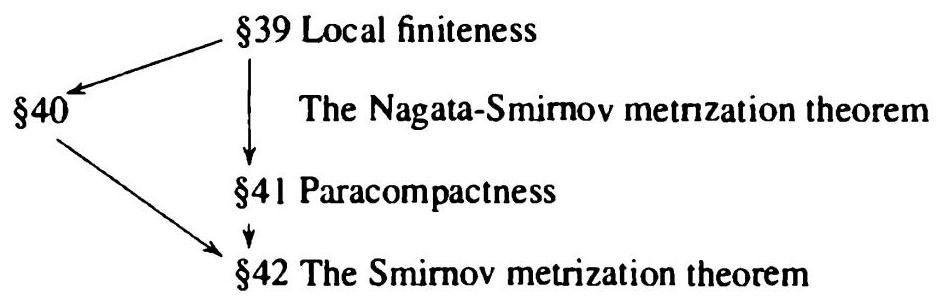
\includegraphics[width=0.8\textwidth]{images/38.1.jpg}
\end{center}
\hspace*{3em} 

\section*{§ 39 Local Finiteness}

In this sections we prove some elementary properties of \idx{locally finite collection}s and a crucial lemma about metrizable spaces.

\begin{definition}
	Let \(X\) be a topological space. A collection \(\mathcal{A}\) of subsets of \(X\) is said to be locally finite in \(X\) if every point of \(X\) has a neighborhood that intersects only finitely many elements of \(\mathcal{A}\)
\end{definition}

\begin{centeredblock}
\begin{example}
	The collection of intervals

\[
\mathcal{A} = \{ \left( {n,n + 2}\right)  \mid  n \in  \mathbb{Z}\}
\]

is locally finite in the topological space \(\mathbb{R}\) , as you can check. On the other hand, the collection

\[
\mathcal{B} = \left\{  {\left( {0,1/n}\right)  \mid  n \in  {\mathbb{Z}}_{ + }}\right\}
\]

is locally finite in(0,1)but not in \(\mathbb{R}\) , as is the collection

\[
\mathcal{C} = \left\{  {\left( {1/\left( {n + 1}\right) ,1/n}\right)  \mid  n \in  {\mathbb{Z}}_{ + }}\right\}
\]
\end{example}
\end{centeredblock}

\begin{lemma}
	Let \(\mathcal{A}\) be a locally finite collection of subsets of \(X\) . Then:

(a) Any subcollection of \(\mathcal{A}\) is locally finite.

(b) The collection \(\mathcal{B} = \{ \bar{A}{\} }_{A \in  \mathcal{A}}\) of the closures of the elements of \(\mathcal{A}\) is locally finite.

(c) \(\overline{\mathop{\bigcup }\limits_{{A \in  \mathcal{A}}}A} = \mathop{\bigcup }\limits_{{A \in  \mathcal{A}}}\overline{A}\) .
\end{lemma}

\begin{proof}
	Statement (a) is trivial. To prove (b), note that any open set \(U\) that intersects the set \(\bar{A}\) necessarily intersects \(A\) . Therefore, if \(U\) is a neighborhood of \(x\) that intersects only finitely many elements \(A\) of \(\mathcal{A}\) , then \(U\) can intersect at most the same number of sets of the collection \(\mathcal{B}\) . (It might intersect fewer sets of \(\mathcal{B}\) , since \({\bar{A}}_{1}\) and \({\bar{A}}_{2}\) can be equal even though \({A}_{1}\) and \({A}_{2}\) are not).
To prove (c), let \(Y\) denote the union of the elements of \(\mathcal{A}\) :

\[
\mathop{\bigcup }\limits_{{A \in  A}}A = Y
\]

In general, \(\bigcup \bar{A} \subset  \bar{Y}\) ; we prove the reverse inclusion, under the assumption of local finiteness. Let \(x \in  \bar{Y}\) ; let \(U\) be a neighborhood of \(x\) that intersects only finitely many elements of \(\mathcal{A}\) , say \({A}_{1},\ldots ,{A}_{k}\) . We assert that \(x\) belongs to one of the sets \({\bar{A}}_{1}\) , \(\ldots ,{\bar{A}}_{k}\) , and hence belongs to \(\bigcup \bar{A}\) . For otherwise, the set \(U - {\bar{A}}_{1} - \cdots  - {\bar{A}}_{k}\) would be a neighborhood of \(x\) that intersects no element of \(\mathcal{A}\) and hence does not intersect \(Y\) , contrary to the assumption that \(x \in  \bar{Y}\) .

There is an analogous concept of local finiteness for an indexed family of subsets of \(X\) . The indexed family \({\left\{  {A}_{\alpha }\right\}  }_{\alpha  \in  J}\) is said to be a locally finite indexed family in \(X\) if every \(x \in  X\) has a neighborhood that intersects \({A}_{\alpha }\) for only finitely many values of \(\alpha\) . What is the relation between the two formulations of local finiteness? It is easy to see that \({\left\{  {A}_{\alpha }\right\}  }_{\alpha  \in  J}\) is a locally finite indexed family if and only if it is locally finite as a collection of sets and each nonempty subset \(A\) of \(X\) equals \({A}_{\alpha }\) for at most finitely many values of \(\alpha\) .

We shall be concerned with locally finite indexed families only in §41, when we deal with partitions of unity.
\end{proof}
\begin{definition}
	A collection \(\mathcal{B}\) of subsets of \(X\) is said to be countably locally finite if \(\mathcal{B}\) can be written as the countable union of collections \({\mathcal{B}}_{n}\) , each of which is locally finite.
\end{definition}

Most authors use the term `` \(\sigma\) -locally finite'' for this concept. The \(\sigma\) comes from measure theory and stands for the phrase ``countable union of `` Note that both a countable collection and a locally finite collection are countably locally finite.

\begin{definition}
	Let \(\mathcal{A}\) be a collection of subsets of the space \(X\) . A collection \(\mathcal{B}\) of subsets of \(X\) is said to be a \idx{refinement} of \(\mathcal{A}\) (or is said to refine \(\mathcal{A}\) ) if for each element \(B\) of \(\mathcal{B}\) , there is an element \(A\) of \(\mathcal{A}\) containing \(B\) . If the elements of \(\mathcal{B}\) are open sets, we call \(\mathcal{B}\) an \idx{open refinement} of \(\mathcal{A}\) ; if they are closed sets, we call \(\mathcal{B}\) a \idx{closed refinement}
\end{definition}

\begin{lemma}
	Let \(X\) be a metrizable space. If \(\mathcal{A}\) is an open covering of \(X\) , then there is an open covering \(\mathcal{E}\) of \(X\) refining \(\mathcal{A}\) that is countably locally finite.
\end{lemma}

\begin{proof}
	We shall use the well-ordering theorem in proving this theorem. Choose a well-ordering \(<\) for the collection \(\mathcal{A}\) . Let us denote the elements of \(\mathcal{A}\) generically by the letters \(U,V,W,\ldots\) .
Choose a metric for \(X\) . Let \(n\) be a positive integer, fixed for the moment. Given an element \(U\) of \(\mathcal{A}\) , let us define \({S}_{n}\left( U\right)\) to be the subset of \(U\) obtained by ``shrinking'' \(U\) a distance of \(1/n\) . More precisely, let

\[
{S}_{n}\left( U\right)  = \{ x \mid  B\left( {x,1/n}\right)  \subset  U\} .
\]

(It happens that \({S}_{n}\left( U\right)\) is a closed set, but that is not important for our purposes.) Now we use the well-ordering \(<\) of \(\mathcal{A}\) to pass to a still smaller set. For each \(U\) in \(\mathcal{A}\) , define

\[
{T}_{n}\left( U\right)  = {S}_{n}\left( U\right)  - \mathop{\bigcup }\limits_{{V < U}}V
\]

The situation where \(\mathcal{A}\) consists of the three sets \(U < V < W\) is pictured in Figure 39.1. Just as the figure suggests, the sets we have formed are disjoint.

\begin{center}
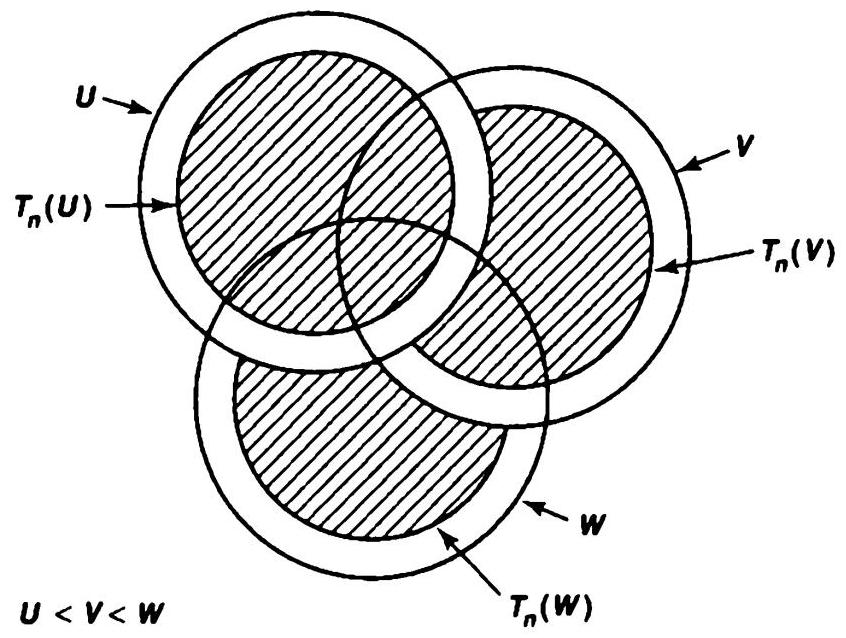
\includegraphics[width=0.7\textwidth]{images/39.1.jpg}
\end{center}
\hspace*{3em} 

Figure 39.1

In fact, they are separated by a distance of at least \(1/n\) . This means that if \(V\) and \(W\) are distinct elements of \(\mathcal{A}\) , then \(d\left( {x,y}\right)  \geq  1/n\) whenever \(x \in  {T}_{n}\left( V\right)\) and \(y \in  {T}_{n}\left( W\right)\) .

To prove this fact, assume the notation has been so chosen that \(V < W\) . Since \(x\) is in \({T}_{n}\left( V\right)\) , then \(x\) is in \({S}_{n}\left( V\right)\) , so the \(1/n\) -neighborhood of \(x\) lies in \(V\) . On the other hand, since \(V < W\) and \(y\) is in \({T}_{n}\left( W\right)\) , the definition of the latter set tells us that \(y\) is not in \(V\) . It follows that \(y\) is not in the \(1/n\) -neighborhood of \(x\) .

The sets \({T}_{n}\left( U\right)\) are not yet the ones we want, for we do not know that they are open sets. (In fact, they are closed.) So let us expand each of them slightly to obtain an open set \({E}_{n}\left( U\right)\) . Specifically, let \({E}_{n}\left( U\right)\) be the \(1/{3n}\) -neighborhood of \({T}_{n}\left( U\right)\) ; that is, let \({E}_{n}\left( U\right)\) be the union of the open balls \(B\left( {x,1/{3n}}\right)\) , for \(x \in  {T}_{n}\left( U\right)\)

In the case \(U < V < W\) , we have the situation pictured in Figure 39.2. As the figure suggests, the sets we have formed are disjoint. Indeed, if \(V\) and \(W\) are distinct elements of \(\mathcal{A}\) , we assert that \(d\left( {x,y}\right)  \geq  1/{3n}\) whenever \(x \in  {E}_{n}\left( V\right)\) and \(y \in  {E}_{n}\left( W\right)\) ; this fact follows at once from the triangle inequality. Note that for each \(V \in  \mathcal{A}\) , the set \({E}_{n}\left( V\right)\) is contained in \(V\) .

\begin{center}
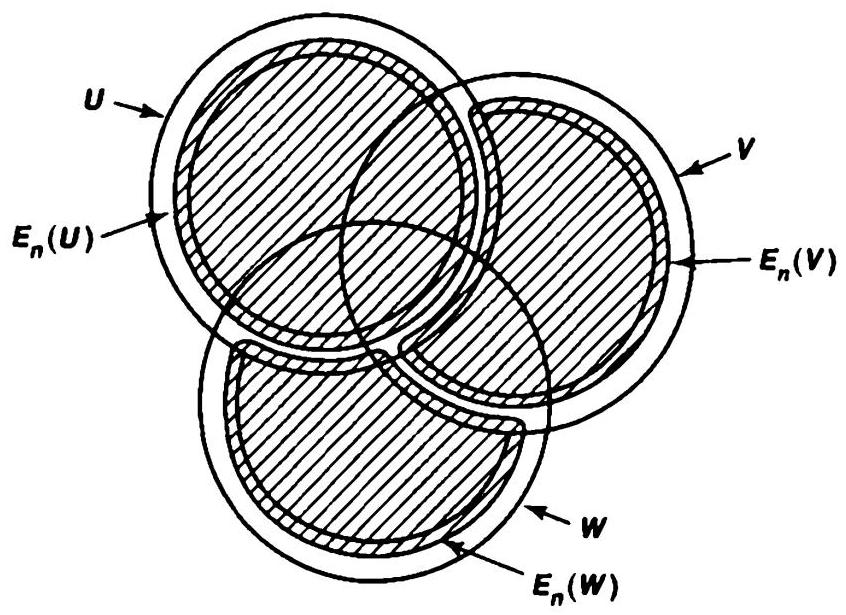
\includegraphics[width=0.7\textwidth]{images/39.2.jpg}
\end{center}
\hspace*{3em} 

Figure 39.2

Now let us define

\[
{\mathcal{E}}_{n} = \left\{  {{E}_{n}\left( U\right)  \mid  U \in  \mathcal{A}}\right\}
\]

We claim that \({\mathcal{E}}_{n}\) is a locally finite collection of open sets that refines \(\mathcal{A}\) . The fact that \({\mathcal{E}}_{n}\) refines \(\mathcal{A}\) comes from the fact that \({E}_{n}\left( V\right)  \subset  V\) for each \(V \in  \mathcal{A}\) . The fact that \({\mathcal{E}}_{n}\) is locally finite comes from the fact that for any \(x\) in \(X\) , the \(1/{6n}\) -neighborhood of \(x\) can intersect at most one element of \({\mathcal{E}}_{n}\) .

Of course, the collection \({\mathcal{E}}_{n}\) , will not cover \(X\) . (Figure 39 2 illustrates that fact.) But we assert that the collection

\[
\varepsilon  = \mathop{\bigcup }\limits_{{n \in  {\mathbb{Z}}_{ + }}}{\varepsilon }_{n}
\]

does cover \(X\) .

Let \(x\) be a point of \(X\) . The collection \(\mathcal{A}\) with which we began covers \(X\) ; let us choose \(U\) to be the first element of \(\mathcal{A}\) (in the well-ordering \(<\) ) that contains \(x\) . Since \(U\) is open, we can choose \(n\) so that \(B\left( {x,1/n}\right)  \subset  U\) Then, by definition, \(x \in  {S}_{n}\left( U\right)\) . Now because \(U\) is the first element of \(\mathcal{A}\) that contains \(x\) , the point \(x\) belongs to \({T}_{n}\left( U\right)\) . Then \(x\) also belongs to the element \({E}_{n}\left( U\right)\) of \({\mathcal{E}}_{n}\) , as desired.
\end{proof}
\section*{Exercises}
\begin{enumerate}[itemsep=0.4em, parsep=0pt, topsep=0pt, partopsep=0pt, leftmargin=*, label=\arabic*., ref=\arabic*]
\item Check the statements in Example 1.
\item Find a \idx{Point-finite collection} point-finite open covering \(\mathcal{A}\) of \(\mathbb{R}\) that is not locally finite. (The collection \(\mathcal{A}\) is point-finite if each point of \(\mathbb{R}\) lies in only finitely many elements of \(\mathcal{A}\) .)
\item Give an example of a collection of sets \(\mathcal{A}\) that is not locally finite, such that the collection \(\mathcal{B} = \{ \bar{A} \mid  A \in  \mathcal{A}\}\) is locally finite.
\item Let \(\mathcal{A}\) be the following collection of subsets of \(\mathbb{R}\) : \[ A = \{ \left( {n,n + 2}\right)  \mid  n \in  \mathbb{Z}\} \] Which of the following collections refine \(\mathcal{A}\) ? \[ \mathcal{B} = \{ \left( {x,x + 1}\right)  \mid  x \in  \mathbb{R}\} , \] \[ \mathcal{C} = \left\{  {\left( {n,n + \frac{3}{2}}\right)  \mid  n \in  \mathbb{Z}}\right\}  , \] \[ \mathcal{D} = \left\{  {\left( {x,x + \frac{3}{2}}\right)  \mid  x \in  \mathbb{R}}\right\}  . \]
\item Show that if \(X\) has a countable basis, a collection \(\mathcal{A}\) of subsets of \(X\) is countably locally finite if and only if it is countable
\item Consider \({\mathbb{R}}^{\omega }\) in the uniform topology. Given \(n\) , let \({\mathcal{B}}_{n}\) be the collection of all subsets of \({\mathbb{R}}^{\omega }\) of the form \(\prod {A}_{i}\) , where \({A}_{i} = \mathbb{R}\) for \(i \leq  n\) and \({A}_{i}\) equals either \(\{ 0\}\) or \(\{ 1\}\) otherwise. Show that the collection \(\mathcal{B} = \bigcup {\mathcal{B}}_{n}\) is countably locally finite, but neither countable nor locally finite.
\end{enumerate}
\section*{§ 40 The Nagata-Smirnov Metrization Theorem}

Now we prove that regularity of \(X\) and the existence of a countably locally finite basis for \(X\) are equivalent to metrizability of \(X\) .

The proof that these conditions imply metrizability follows very closely the second proof we gave of the Urysohn metrization theorem. In that proof we constructed a map of the space \(X\) into \({\mathbb{R}}^{\omega }\) that was an imbedding relative to the uniform metric \(\widetilde{\rho }\) on \({\mathbb{R}}^{\omega }\) . So let us review the major elements of that proof. The first step of the proof was to prove that every regular space \(X\) with a countable basis is normal. The second step was to construct a countable collection \(\left\{  {f}_{n}\right\}\) of real-valued functions on \(X\) that separated points from closed sets. The third step was to use the functions \({f}_{n}\) to define a map imbedding \(X\) in the product space \({\mathbb{R}}^{\omega }\) . And the fourth step was to show that if \({f}_{n}\left( x\right)  \leq  1/n\) for all \(x\) , then this map actually imbeds \(X\) in the metric space \(\left( {{\mathbb{R}}^{\omega },\bar{\rho }}\right)\) .

Each of these steps needs to be generalized in order to prove the general metrization theorem. First, we show that a regular space \(X\) with a basis that is countably locally finite is normal. Second, we construct a certain collection of real-valued functions \(\left\{  {f}_{\alpha }\right\}\) on \(X\) that separates points from closed sets. Third, we use these functions to imbed \(X\) in the product space \({\mathbb{R}}^{J}\) , for some \(J\) . And fourth, we show that if the functions \({f}_{\alpha }\) are sufficiently small, this map actually imbeds \(X\) in the metric space \(\left( {{\mathbb{R}}^{J},\bar{\rho }}\right)\)

Before we start, we need to recall a notion we have already introduced in the exercises, that of a \({G}_{\delta }\) set.

\begin{definition}
	A subset \(A\) of a space \(X\) is called a \({G}_{\delta }\) set in \(X\) if it equals the intersection of a countable collection of open subsets of \(X\) .
\end{definition}

\begin{centeredblock}
\begin{example}
	Each open subset of \(X\) is a \({G}_{\delta }\) set, invially In a first-countable Hausdorff space, each one-point set is a \({G}_{\delta }\) set The one-point subset \(\{ \Omega \}\) of \({\bar{S}}_{\Omega }\) is not a \({G}_{\delta }\) set, as you can check
\end{example}
\end{centeredblock}

\begin{centeredblock}
\begin{example}
	In a metric space \(X\) , each closed set is a \({G}_{\delta }\) set. Given \(A \subset  X\) , let \(U\left( {A,\epsilon }\right)\) denote the \(\epsilon\) -neighborhood of \(A\) If \(A\) is closed, you can check that

\[
A = \mathop{\bigcap }\limits_{{n \in  {\mathbb{Z}}_{ + }}}U\left( {A,1/n}\right)
\]
\end{example}
\end{centeredblock}

\begin{lemma}
	Let \(X\) be a regular space with a basis \(\mathcal{B}\) that is countably locally finite. Then \(X\) is normal, and every closed set in \(X\) is a \({G}_{\delta }\) set in \(X\) .
\end{lemma}

\begin{proof}
	Step 1. Let \(W\) be open in \(X\) . We show there is a countable collection \(\left\{  {U}_{n}\right\}\) of open sets of \(X\) such that
\[
W = \bigcup {U}_{n} = \bigcup {\bar{U}}_{n}
\]

Since the basis \(\mathcal{B}\) for \(X\) is countably locally finite, we can write \(\mathcal{B} = \bigcup {\mathcal{B}}_{n}\) , where each collection \({\mathcal{B}}_{n}\) is locally finite. Let \({\mathcal{C}}_{n}\) be the collection of those basis elements \(B\) such that \(B \in  {\mathcal{B}}_{n}\) and \(\bar{B} \subset  W\) . Then \({\mathcal{C}}_{n}\) is locally finite, being a subcollection of \({\mathcal{B}}_{n}\) Define

\[
{U}_{n} = \mathop{\bigcup }\limits_{{B \in  {\mathcal{C}}_{n}}}B
\]

Then \({U}_{n}\) is an open set, and by Lemma 39 1,

\[
{\bar{U}}_{n} = \mathop{\bigcup }\limits_{{B \in  {\mathcal{C}}_{n}}}\bar{B}.
\]

Therefore, \({\bar{U}}_{n} \subset  W\) , so that

\[
\bigcup {U}_{n} \subset  \bigcup {\bar{U}}_{n} \subset  W
\]

We assert that equality holds. Given \(x \in  W\) , there is by regularity a basis element \(B \in  \mathcal{B}\) such that \(x \in  B\) and \(\bar{B} \subset  W\) . Now \(B \in  {\mathcal{B}}_{n}\) for some \(n\) . Then \(B \in  {\mathcal{C}}_{n}\) by definition, so that \(x \in  {U}_{n}\) . Thus \(W \subset  \bigcup {U}_{n}\) , as desired.

Step 2. We show that every closed set \(C\) in \(X\) is a \({G}_{\delta }\) set in \(X\) Given \(C\) , let \(W = X - C\) . By Step 1, there are sets \({U}_{n}\) in \(X\) such that \(W = \bigcup {U}_{n}\) Then

\[
C = \bigcap \left( {X - {\bar{U}}_{n}}\right)
\]

so that \(C\) equals a countable intersection of open sets of \(X\) .

Step 3. We show \(X\) is normal Let \(C\) and \(D\) be disjoint closed sets in \(X\) . Applying Step 1 to the open set \(X - D\) , we construct a countable collection \(\left\{  {U}_{n}\right\}\) of open sets such that \(\mathop{\bigcup }\limits_{n}{U}_{n} = \mathop{\bigcup }\limits_{n}{\bar{U}}_{n} = X - D\) . Then \(\left\{  {U}_{n}\right\}\) covers \(C\) and each set \({\bar{U}}_{n}\) is disjoint from \(D\) . Similarly, there is a countable covering \(\left\{  {V}_{n}\right\}\) of \(D\) by open sets whose closures are disjoint from \(C\) .

Now we are back in the situation that arose in the proof that a regular space with a countable basis is normal (Theorem 32.1). We can repeat that proof verbatim. Define

\[
{U}_{n}^{\prime } = {U}_{n} - \mathop{\bigcup }\limits_{{i = 1}}^{n}{\bar{V}}_{i}\;\text{ and }\;{V}_{n}^{\prime } = {V}_{n} - \mathop{\bigcup }\limits_{{i = 1}}^{n}{\bar{U}}_{i}
\]

Then the sets

\[
{U}^{\prime } = \mathop{\bigcup }\limits_{{n \in  {\mathbb{Z}}_{ + }}}{U}_{n}^{\prime }\;\text{ and }\;{V}^{\prime } = \mathop{\bigcup }\limits_{{n \in  {\mathbb{Z}}_{ + }}}{V}_{n}^{\prime }
\]

are disjoint open sets about \(C\) and \(D\) , respectively.
\end{proof}
\begin{lemma}
	Let \(X\) be normal; let \(A\) be a closed \({G}_{\delta }\) set in \(X\) . Then there is a continuous function \(f : X \rightarrow  \left\lbrack  {0,1}\right\rbrack\) such that \(f\left( x\right)  = 0\) for \(x \in  A\) and \(f\left( x\right)  > 0\) for \(x \notin  A\) .
\end{lemma}

\begin{proof}
	We gave this as an exercise in \(\$ {33}\) , we provide a proof here. Write \(A\) as the intersection of the open sets \({U}_{n}\) , for \(n \in  {\mathbb{Z}}_{ + }\) For each \(n\) , choose a continuous function \({f}_{n} : X \rightarrow  \left\lbrack  {0,1}\right\rbrack\) such that \(f\left( x\right)  = 0\) for \(x \in  A\) and \(f\left( x\right)  = 1\) for \(x \in  X - {U}_{n}\) Define \(f\left( x\right)  = \sum {f}_{n}\left( x\right) /{2}^{n}\) The series converges uniformly, by comparison with \(\sum 1/{2}^{n}\) , so that \(f\) is continuous. Also, \(f\) vanishes on \(A\) and is positive on \(X - A\)
\end{proof}
\begin{theorem}[\idx{Nagata-Smirnov metrization theorem}]
	A space \(X\) is metrizable if and only if \(X\) is regular and has a basis that is countably locally finite.
\end{theorem}

\begin{proof}
	Step 1. Assume \(X\) is regular with a countably locally finite basis \(\mathcal{B}\) Then \(X\) is normal, and every closed set in \(X\) is a \({G}_{\delta }\) set in \(X\) . We shall show that \(X\) is metrizable by imbedding \(X\) in the metric space \(\left( {{\mathbb{R}}^{J},\bar{\rho }}\right)\) for some \(J\)
Let \(\mathcal{B} = \bigcup {\mathcal{B}}_{n}\) , where each collection \({\mathcal{B}}_{n}\) is locally finite. For each positive integer \(n\) , and each basis element \(B \in  {\mathcal{B}}_{n}\) , choose a continuous function

\[
{f}_{n,B} : X \rightarrow  \left\lbrack  {0,1/n}\right\rbrack
\]

such that \({f}_{n,B}\left( x\right)  > 0\) for \(x \in  B\) and \({f}_{n,B}\left( x\right)  = 0\) for \(x \notin  B\) . The collection \(\left\{  {f}_{n,B}\right\}\) separates points from closed sets in \(X\) . Given a point \({x}_{0}\) and a neighborhood \(U\) of \({x}_{0}\) , there is a basis element \(B\) such that \({x}_{0} \in  B \subset  U\) . Then \(B \in  {\mathcal{B}}_{n}\) for some \(n\) , so that \({f}_{n,B}\left( {x}_{0}\right)  > 0\) and \({f}_{n,B}\) vanishes outside \(U\) .

Let \(J\) be the subset of \({\mathbb{Z}}_{ + } \times  \mathcal{B}\) consisting of all pairs(n, B)such that \(B\) is an element of \({\mathcal{B}}_{n}\) . Define

\[
F : X \rightarrow  {\left\lbrack  0,1\right\rbrack  }^{J}
\]

by the equation

\[
F\left( x\right)  = \left( {{f}_{n,B}\left( x\right) }\right) \left( {n,b}\right)  \in  J.
\]

Relative to the product topology on \({\left\lbrack  0,1\right\rbrack  }^{J}\) , the map \(F\) is an imbedding, by Theorem 34.2.

Now we give \({\left\lbrack  0,1\right\rbrack  }^{J}\) the topology induced by the uniform metric and show that \(F\) is an imbedding relative to this topology as well. Here is where the condition \({f}_{n,B}\left( x\right)  < 1/n\) comes in. The uniform topology is finer (larger) than the product topology. Therefore, relative to the uniform metric, the map \(F\) is injective and carries open sets of \(X\) onto open sets of the image space \(Z = F\left( X\right)\) We must give a separate proof that \(F\) is continuous.

Note that on the subspace \({\left\lbrack  0,1\right\rbrack  }^{J}\) of \({\mathbb{R}}^{J}\) , the uniform metric equals the metric

\[
\rho \left( {\left( {x}_{\alpha }\right) ,\left( {y}_{\alpha }\right) }\right)  = \sup \left\{  \left| {{x}_{\alpha } - {y}_{\alpha }}\right| \right\}  .
\]

To prove continuity, we take a point \({x}_{0}\) of \(X\) and a number \(\epsilon  > 0\) , and find a neighborhood \(W\) of \({x}_{0}\) such that

\[
x \in  W \Rightarrow  \rho \left( {F\left( x\right) ,F\left( {x}_{0}\right) }\right)  < \epsilon
\]

Let \(n\) be fixed for the moment. Choose a neighborhood \({U}_{n}\) of \({x}_{0}\) that intersects only finitely many elements of the collection \({\mathcal{B}}_{n}\) . This means that as \(B\) ranges over \({\mathcal{B}}_{n}\) , all but finitely many of the functions \({f}_{n,B}\) are identically equal to zero on \({U}_{n}\) . Because each function \({f}_{n,B}\) is continuous, we can now choose a neighborhood \({V}_{n}\) of \({x}_{0}\) contained in \({U}_{n}\) on which each of the remaining functions \({f}_{n,B}\) , for \(B \in  {\mathcal{B}}_{n}\) , varies by at most \(\epsilon /2\) .

Choose such a neighborhood \({V}_{n}\) of \({x}_{0}\) for each \(n \in  {\mathbb{Z}}_{ + }\) . Then choose \(N\) so that \(1/N \leq  \epsilon /2\) , and define \(W = {V}_{1} \cap  \cdots  \cap  {V}_{N}\) We assert that \(W\) is the desired neighborhood of \({x}_{0}\) . Let \(x \in  W\) . If \(n \leq  N\) , then

\[
\left| {{f}_{n,B}\left( x\right)  - {f}_{n,B}\left( {x}_{0}\right) }\right|  \leq  \epsilon /2
\]

because the function \({f}_{n,B}\) either vanishes identically or varies by at most \(\epsilon /2\) on \(W\) . If \(n > N\) , then

\[
\left| {{f}_{n,B}\left( x\right)  - {f}_{n,B}\left( {x}_{0}\right) }\right|  \leq  1/n < \epsilon /2
\]

because \({f}_{n,B}\) maps \(X\) into \(\left\lbrack  {0,1/n}\right\rbrack\) . Therefore,

\[
\rho \left( {F\left( x\right) ,F\left( {x}_{0}\right) }\right)  \leq  \epsilon /2 < \epsilon ,
\]

as desired.

Step 2. Now we prove the converse. Assume \(X\) is metrizable. We know \(X\) is regular; let us show that \(X\) has a basis that is countably locally finite.

Choose a metric for \(X\) . Given \(m\) , let \({A}_{m}\) be the covering of \(X\) by all open balls of radius \(1/m\) . By Lemma 39.2, there is an open covering \({\mathcal{B}}_{m}\) of \(X\) refining \({\mathcal{A}}_{m}\) such that \({\mathcal{B}}_{m}\) is countably locally finite. Note that each element of \({\mathcal{B}}_{m}\) has diameter at most \(2/m\) Let \(\mathcal{B}\) be the union of the collections \({\mathcal{B}}_{m}\) , for \(m \in  {\mathbb{Z}}_{ + }\) . Because each collection \({\mathcal{B}}_{m}\) is countably locally finite, so is \(\mathcal{B}\) . We show that \(\mathcal{B}\) is a basis for \(X\) .

Given \(x \in  X\) and given \(\epsilon  > 0\) , we show that there is an element \(B\) of \(\mathcal{B}\) containing \(x\) that is contained in \(B\left( {x,\epsilon }\right)\) . First choose \(m\) so that \(1/m < \epsilon /2\) . Then, because \({\mathcal{B}}_{m}\) covers \(X\) , we can choose an element \(B\) of \({\mathcal{B}}_{m}\) that contains \(x\) . Since \(B\) contains \(x\) and has diameter at most \(2/m < \epsilon\) , it is contained in \(B\left( {x,\epsilon }\right)\) , as desired.
\end{proof}
\section*{Exercises}
\begin{enumerate}[itemsep=0.4em, parsep=0pt, topsep=0pt, partopsep=0pt, leftmargin=*, label=\arabic*., ref=\arabic*]
\item Check the details of Examples 1 and 2.
\item A subset \(W\) of \(X\) is said to be an `` \({F}_{\sigma }\) set'' in \(X\) if \(W\) equals a countable union of closed sets of \(X\) . Show that \(W\) is an \({F}_{\sigma }\) set in \(X\) if and only if \(X - W\) is a \({G}_{\delta }\) set in \(X\) . [The termunology comes from the French. The ``F'' stands for ``fermé,'' which means ``closed,'' and the `` \(\sigma\) `` for ``somme,'' which means ``union.'']
\item Many spaces have countable bases; but no \({T}_{1}\) space has a locally finite basis unless it is discrete. Prove this fact.
\item Find a nondiscrete space that has a countably locally finite basis but does not have a countable basis.
\item A collection \(\mathcal{A}\) of subsets of \(X\) is said to be \idx{locally discrete} if each point of \(X\) has a neighborhood that intersects at most one element of \(\mathcal{A}\) . A collection \(\mathcal{B}\) is \idx{countably locally discrete} (or `` \(\sigma\) -locally discrete'') if it equals a countable union of locally discrete collections. Prove the following: \textsl{Theorem. (\idx{Bing metrization theorem}).} A space \(X\) is metrizable if and only if it is regular and has a basis that is countably locally discrete. 
\end{enumerate}
\section*{§ 41 Paracompactness}

The concept of paracompactness is one of the most useful generalizations of compactness that has been discovered in recent years. It is particularly useful for applications in topology and differential geometry We shall give just one application, a metrization theorem that we prove in the next section.

Many of the spaces that are familiar to us already are paracompact. For instance, every compact space is paracompact, this will be an immediate consequence of the definition. It is also true that every metrizable space is paracompact, this is a theorem due to A. H. Stone, which we shall prove. Thus the class of \idx{paracompact space}s includes the two most important classes of spaces we have studied. It includes many other spaces as well.

To see how paracompactness generalizes compactness, we recall the definition of compactness: A space \(X\) is said to be compact if every open covering \(\mathcal{A}\) of \(X\) contains a finite subcollection that covers \(X\) . An equivalent way of saying this is the following:

A space \(X\) is compact if every open covering \(\mathcal{A}\) of \(X\) has a finite open refinement \(\mathcal{B}\) that covers \(X\)

This definition is equivalent to the usual one, given such a refinement \(\mathcal{B}\) , one can choose for each element of \(\mathcal{B}\) an element of \(\mathcal{A}\) containing it; in this way one obtains a finite subcollection of \(\mathcal{A}\) that covers \(X\) .

This new formulation of compactness is an awkward one, but it suggests a way to generalize.

\begin{definition}
	A space \(X\) is paracompact if every open covering \(\mathcal{A}\) of \(X\) has a locally finite open refinement \(\mathcal{B}\) that covers \(X\) .
\end{definition}

Many authors, following the lead of Bourbaki, include as part of the definition of the term paracompact the requirement that the space be Hausdorff. (Bourbaki also includes the Hausdorff condition as part of the definition of the term compact.) We shall not follow this convention.

\begin{centeredblock}
\begin{example}
	The space \({\mathbb{R}}^{n}\) is paracompact Let \(X = {\mathbb{R}}^{n}\) Let \(\mathcal{A}\) be an open covering of \(X\) . Let \({B}_{0} = \varnothing\) , and for each positive integer \(m\) , let \({B}_{m}\) denote the open ball of radius \(m\) centered at the origin. Given \(m\) , choose finitely many elements of \(\mathcal{A}\) that cover \({\widetilde{B}}_{m}\) and intersect each one with the open set \(X - {\bar{B}}_{m - 1}\) , let this finite collection of open sets be denoted \({\mathcal{C}}_{m}\) Then the collection \(\mathcal{C} = \bigcup {\mathcal{C}}_{m}\) is a refinement of \(\mathcal{A}\) It is clearly locally finite, for the open set \({B}_{m}\) intersects only finitely many elements of \(\mathcal{C}\) , namely those elements beloriging to the collection \({\mathcal{C}}_{1} \cup  \; \cup  {\mathcal{C}}_{m}\) . Finally, \(\mathcal{C}\) covers \(X\) For, given \(x\) , let \(m\) be the smallest integer such that \(x \in  {\bar{B}}_{m}\) . Then \(x\) belongs to an element of \({\mathcal{C}}_{m}\) , by definition.
\end{example}
\end{centeredblock}

Some of the properties of a paracompact space are similar to those of a compact space. For instance, a subspace of a paracompact space is not necessarily paracompact; but a closed subspace is paracompact. Also, a paracompact Hausdorff space is normal. In other ways, a paracompact space is not similar to a compact space; in particular, the product of two paracompact spaces need not be paracompact. We shall verify these facts shortly.

\section*{Theorem 41.1. Every paracompact Hausdorff space \(X\) is normal}

Proof The proof is somewhat similar to the proof that a compact Hausdorff space is normal.

First one proves regularity Let \(a\) be a point of \(X\) and let \(B\) be a closed set of \(X\) disjoint from \(a\) . The Hausdorff condition enables us to choose, for each \(b\) in \(B\) , an open set \({U}_{b}\) about \(b\) whose closure is disjoint from \(a\) . Cover \(X\) by the open sets \({U}_{b}\) , along with the open set \(X - B\) ; take a locally finite open refinement \(\mathcal{C}\) that covers \(X\) . Form the subcollection \(\mathcal{D}\) of \(\mathcal{C}\) consisting of every element of \(\mathcal{C}\) that intersects \(B\) . Then \(\mathcal{D}\) covers \(B\) . Furthermore, if \(D \in  \mathcal{D}\) , then \(\bar{D}\) is disjoint from \(a\) . For \(D\) intersects \(B\) , so it lies in some set \({U}_{b}\) , whose closure is disjoint from \(a\) . Let

\[
V = \mathop{\bigcup }\limits_{{D \in  \mathcal{D}}}D
\]

then \(V\) is an open set in \(X\) containing \(B\) . Because \(\mathcal{D}\) is locally finite,

\[
\bar{V} = \mathop{\bigcup }\limits_{{D \in  \mathcal{D}}}\bar{D}
\]

so that \(\bar{V}\) is disjoint from \(a\) . Thus regularity is proved.

To prove normality, one merely repeats the same argument, replacing \(a\) by the closed set \(A\) throughout and replacing the Hausdorff condition by regularity.

\section*{Theorem 41.2. Every closed subspace of a paracompact space is paracompact.}

\begin{proof}
	Let \(Y\) be a closed subspace of the paracompact space \(X\) ; let \(\mathcal{A}\) be a covering of \(Y\) by sets open in \(Y\) . For each \(A \in  \mathcal{A}\) , choose an open set \({A}^{\prime }\) of \(X\) such that \({A}^{\prime } \cap  Y = A\) . Cover \(X\) by the open sets \({A}^{\prime }\) , along with the open set \(X - Y\) . Let \(\mathcal{B}\) be a locally finite open refinement of this covering that covers \(X\) . The collection
\[
\mathcal{C} = \{ B \cap  Y \mid  B \in  \mathcal{B}\}
\]

is the required locally finite open refinement of \(\mathcal{A}\)

\begin{centeredblock}
\begin{example}
	A paracompact subspace of a Hausdorff space X need not be closed in X. Indeed, the open interval(0,1)is paracompact, being homeomorphic to \(\mathbb{R}\) , but it is not closed in \(\mathbb{R}\)
\end{example}
\end{centeredblock}

\begin{centeredblock}
\begin{example}
	A subspace of a paracompact space need not be paracompact The space \({\bar{S}}_{\Omega } \times  {\bar{S}}_{\Omega }\) is compact and, therefore, paracompact. But the subspace \({S}_{\Omega } \times  {\bar{S}}_{\Omega }\) is not para-compact, for it is Hausdorff but not normal.
\end{example}
\end{centeredblock}

To prove the important theorem that every metrizable space is paracompact, we need the following lemma, due to E. Michael, which is also useful for other purposes:
\end{proof}
\begin{lemma}
	Let \(X\) be regular. Then the following conditions on \(X\) are equivalent: Every open covering of \(X\) has a refinement that is:

(1) An open covering of \(X\) and countably locally finite.

(2) A covering of \(X\) and locally finite.

(3) A closed covering of \(X\) and locally finite.

(4) An open covering of \(X\) and locally finite.
\end{lemma}

\begin{proof}
	It is trivial that \(\left( 4\right)  \Rightarrow  \left( 1\right)\) . What we need to prove our theorem is the converse In order to prove the converse, we must go through the steps \(\left( 1\right)  \Rightarrow  \left( 2\right)  \Rightarrow  \left( 3\right)  \Rightarrow  \left( 4\right)\) anyway, so we have for convenience listed these conditions in the statement of the lemma.
(1) \(\Rightarrow\) (2). Let \(\mathcal{A}\) be an open covering of \(X\) . Let \(\mathcal{B}\) be an open refinement of \(\mathcal{A}\) that covers \(X\) and is countably locally finite; let

\[
\mathcal{B} = \bigcup {\mathcal{B}}_{n}
\]

where each \({\mathcal{B}}_{n}\) is locally finite.

Now we apply essentially the same sort of shrinking trick we have used before to make sets from different \({\mathcal{B}}_{n}\) 's disjoint. Given \(i\) , let

\[
{V}_{i} = \mathop{\bigcup }\limits_{{U \in  {\mathcal{B}}_{i}}}U
\]

Then for each \(n \in  {\mathbb{Z}}_{ + }\) and each element \(U\) of \({\mathcal{B}}_{n}\) , define

\[
{S}_{n}\left( U\right)  = U - \mathop{\bigcup }\limits_{{i < n}}{V}_{i}
\]

[Note that \({S}_{n}\left( U\right)\) is not necessarily open, nor closed.] Let

\[
{\mathcal{C}}_{n} = \left\{  {{S}_{n}\left( U\right)  \mid  U \in  {\mathcal{B}}_{n}}\right\}
\]

Then \({\mathcal{C}}_{n}\) is a refinement of \({\mathcal{B}}_{n}\) , because \({S}_{n}\left( U\right)  \subset  U\) for each \(U \in  {\mathcal{B}}_{n}\) .

Let \(\mathcal{C} = \bigcup {\mathcal{C}}_{n}\) . We assert that \(\mathcal{C}\) is the required locally finite refinement of \(\mathcal{A}\) , covering \(X\)

Let \(x\) be a point of \(X\) . We wish to prove that \(x\) lies in an element of \(\mathcal{C}\) , and that \(x\) has a neighborhood intersecting only finitely many elements of \(\mathcal{C}\) . Consider the covering \(\mathcal{B} = \bigcup {\mathcal{B}}_{n}\) ; let \(N\) be the smallest integer such that \(x\) lies in an element of \({\mathcal{B}}_{N}\) . Let \(U\) be an element of \({\mathcal{B}}_{N}\) containing \(x\) . First, note that since \(x\) lies in no element of \({\mathcal{B}}_{i}\) for \(i < N\) , the point \(x\) lies in the element \({S}_{N}\left( U\right)\) of \(\mathcal{C}\) . Second, note that since each collection \({\mathcal{B}}_{n}\) is locally finite, we can choose for each \(n = 1,\ldots ,N\) a neighborhood \({W}_{n}\) of \(x\) that intersects only finitely many elements of \({\mathcal{B}}_{n}\) . Now if \({W}_{n}\) intersects the element \({S}_{n}\left( V\right)\) of \({\mathcal{C}}_{n}\) , it must intersect the element \(V\) of \({\mathcal{B}}_{n}\) , since \({S}_{n}\left( V\right)  \subset  V\) . Therefore, \({W}_{n}\) intersects only finitely many elements of \({\mathcal{C}}_{n}\) . Furthermore, because \(U\) is in \({\mathcal{B}}_{N},U\) intersects no element of \({\mathcal{C}}_{n}\) for \(n > N\) As a result, the neighborhood

\[
{W}_{1} \cap  {W}_{2} \cap  \cdots  \cap  {W}_{N} \cap  U
\]

of \(x\) intersects only finitely many elements of \(\mathcal{C}\) .

\(\left( 2\right)  \Rightarrow  \left( 3\right)\) Let \(\mathcal{A}\) be an open covering of \(X\) . Let \(\mathcal{B}\) be the collection of all open sets \(U\) of \(X\) such that \(\bar{U}\) is contained in an element of \(\mathcal{A}\) . By regularity, \(\mathcal{B}\) covers \(X\) . Using (2), we can find a refinement \(\mathcal{C}\) of \(\mathcal{B}\) that covers \(X\) and is locally finite. Let

\[
\mathcal{D} = \{ \bar{C} \mid  C \in  \mathcal{C}\} .
\]

Then \(\mathcal{D}\) also covers \(X\) ; it is locally finite by Lemma 39.1; and it refines \(\mathcal{A}\) .

\(\left( 3\right)  \Rightarrow  \left( 4\right)\) . Let \(\mathcal{A}\) be an open covering of \(X\) . Using(3), choose \(\mathcal{B}\) to be a refinement of \(\mathcal{A}\) that covers \(X\) and is locally finite (We can take \(\mathcal{B}\) to be a closed refinement if we like, but that is irrelevant.) We seek to expand each element \(B\) of \(\mathcal{B}\) slightly to an open set, making the expansion slight enough that the resulting collection of open sets will still be locally finite and will still refine \(\mathcal{A}\) .

This step involves a new trick. The previous trick, used several times, consisted of ordering the sets in some way and forming a new set by subtracting off all the previous ones. That trick shrinks the sets; to expand them we need something different. We shall introduce an auxiliary locally finite closed covering \(\mathcal{C}\) of \(X\) and use it to expand the elements of \(\mathcal{B}\) .

For each point \(x\) of \(X\) , there is a neighborhood of \(x\) that intersects only finitely many elements of \(\mathcal{B}\) . The collection of all open sets that intersect only finitely many elements of \(\mathcal{B}\) is thus an open covering of \(X\) . Using (3) again, let \(\mathcal{C}\) be a closed refinement of this covering that covers \(X\) and is locally finite. Each element of \(\mathcal{C}\) intersects only finitely many elements of \(\mathcal{B}\) .

For each element \(B\) of \(B\) , let

\[
\mathcal{C}\left( B\right)  = \{ C \mid  C \in  \mathcal{C}\text{ and }C \subset  X - B\}
\]

Then define

\[
E\left( B\right)  = X - \mathop{\bigcup }\limits_{{C \in  C\left( B\right) }}C.
\]

Because \(\mathcal{C}\) is a locally finite collection of closed sets, the union of the elements of any subcollection of \(\mathcal{C}\) is closed, by Lemma 39.1. Therefore, the set \(E\left( B\right)\) is an open set. Furthermore, \(E\left( B\right)  \supset  B\) by definition. (See Figure 41 1, in which the elements of \(\mathcal{B}\) are represented as closed circular regions and line segments, and the elements of \(\mathcal{C}\) are represented as closed square regions.)

\begin{center}
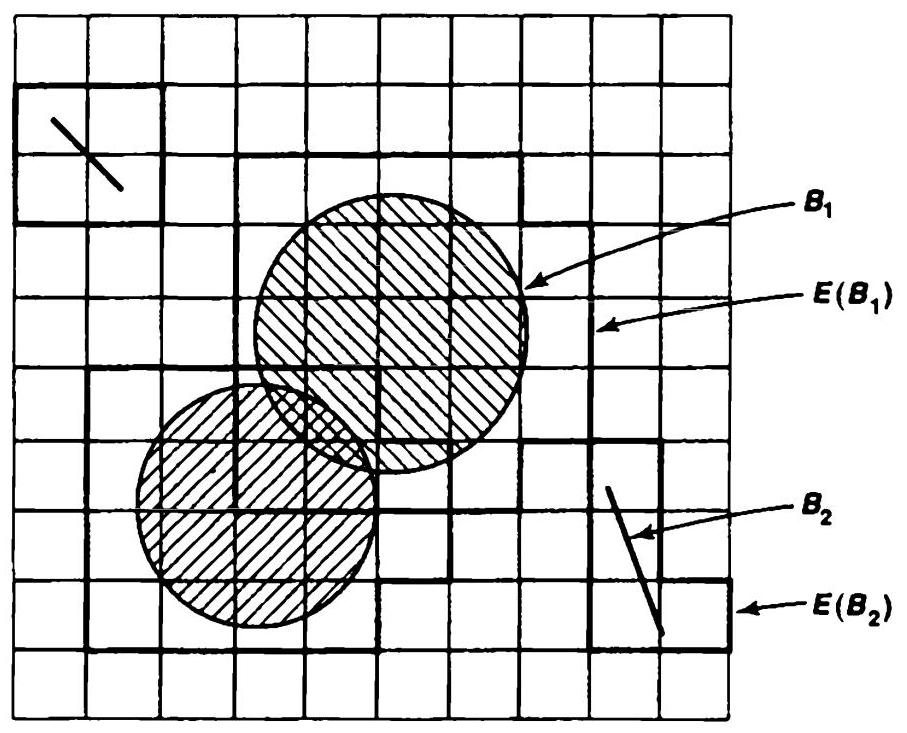
\includegraphics[width=0.8\textwidth]{images/41.1.jpg}
\end{center}
\hspace*{3em} 

Figure 41.1

Now we may have expanded each \(B\) too much; the collection \(\{ E\left( B\right) \}\) may not be a refinement of \(\mathcal{A}\) . This is easily remedied. For each \(B \in  \mathcal{B}\) , choose an element \(F\left( B\right)\) of \(\mathcal{A}\) containing \(B\) . Then define

\[
\mathcal{D} = \{ E\left( B\right)  \cap  F\left( B\right)  \mid  B \in  \mathcal{B}\} .
\]

The collection \(\mathcal{D}\) is a refinement of \(\mathcal{A}\) . Because \(B \subset  \left( {E\left( B\right)  \cap  F\left( B\right) }\right)\) and \(\mathcal{B}\) covers \(X\) , the collection \(\mathcal{D}\) also covers \(X\)

We have finally to prove that \(\mathcal{D}\) is locally finite. Given a point \(x\) of \(X\) , choose a neighborhood \(W\) of \(x\) that intersects only finitely many elements of \(\mathcal{C}\) , say \({C}_{1},\ldots ,{C}_{k}\) We show that \(W\) intersects only finitely many elements of \(\mathcal{D}\) . Because \(\mathcal{C}\) covers \(X\) , the set \(W\) is covered by \({C}_{1},\ldots ,{C}_{k}\) . Thus, it suffices to show that each element \(C\) of \(\mathcal{C}\) intersects only finitely many elements of \(\mathcal{D}\) . Now if \(C\) intersects the set \(E\left( B\right)  \cap  F\left( B\right)\) , then it intersects \(E\left( B\right)\) , so by definition of \(E\left( B\right)\) it is not contained in \(X - B\) , hence \(C\) must intersect \(B\) . Since \(C\) intersects only finitely many elements of \(\mathcal{B}\) , it can intersect at most the same number of elements of the collection \(\mathcal{D}\)
\end{proof}
\section*{Theorem 41.4. Every metrizable space is paracompact}

\begin{proof}
	Let \(X\) be a metrizable space. We already know from Lemma 39.2 that, given an open covering \(\mathcal{A}\) of \(X\) , it has an open refinement that covers \(X\) and is countably locally finite. The preceding lemma then implies that \(\mathcal{A}\) has an open refinement that covers \(X\) and is locally finite
\end{proof}
\begin{theorem}
	Every regular Lindelöf space is paracompact
\end{theorem}

\begin{proof}
	Let \(X\) be regular and Lindelof. Given an open covering \(\mathcal{A}\) of \(X\) , it has a countable subcollection that covers \(X\) , this subcollection is automatically countably locally finite The preceding lemma applies to show \(\mathcal{A}\) has an open refinement that covers \(X\) and is locally finite.
\end{proof}

\begin{centeredblock}
\begin{example}
	The product of two paracompact spaces need not be paracompact The space \({\mathbb{R}}_{\ell }\) is paracompact, for it is regular and Lindelof However, \({\mathbb{R}}_{\ell } \times  {\mathbb{R}}_{\ell }\) is not paracom-pact, for it is Hausdorff but not normal
\end{example}
\end{centeredblock}

\begin{centeredblock}
\begin{example}
	The space \({\mathbb{R}}^{\omega }\) is paracompact in both the product and uniform topologies. This result follows from the fact that \({\mathbb{R}}^{\omega }\) is metrizable in these topologies. It is not known whether \({\mathbf{R}}^{\omega }\) is paracompact in the box topology (See the comment in Exercise 5 of §32 )
\end{example}
\end{centeredblock}

\begin{centeredblock}
\begin{example}
	The product space \({\mathbb{R}}^{J}\) is not paracompact if \(J\) is uncountable For \({\mathbb{R}}^{J}\) is Hausdorff but not normal
\end{example}
\end{centeredblock}

One of the most useful properties that a paracompact space \(X\) possesses has to do with the existence of partitions of unity on \(X\) . We have already seen the finite version of this notion in \(§{36}\) , we discuss the general case now. Recall that if \(\phi : X \rightarrow  \mathbb{R}\) , the support of \(\phi\) is the closure of the set of those \(x\) for which \(\phi \left( x\right)  \neq  0\) .

\begin{definition}
	Let \({\left\{  {U}_{\alpha }\right\}  }_{\alpha  \in  J}\) be an indexed open covering of \(X\) . An indexed family of continuous functions

\[
{\phi }_{\alpha } : X \rightarrow  \left\lbrack  {0,1}\right\rbrack
\]

is said to be a partition of unity on \(X\) , dominated by \(\left\{  {U}_{\alpha }\right\}\) , if:

(1) (Support \({\phi }_{\alpha }\) ) \(\subset  {U}_{\alpha }\) for each \(\alpha\) .

(2) The indexed family \(\left\{  {\text{ Support }{\phi }_{\alpha }}\right\}\) is locally finite

(3) \(\sum {\phi }_{\alpha }\left( x\right)  = 1\) for each \(x\) .
\end{definition}

Condition (2) implies that each \(x \in  X\) has a neighborhood on which the function \({\phi }_{\alpha }\) vanishes identically for all but finitely many values of \(\alpha\) . Thus we can make sense of the ``sum'' indicated in (3); we interpret it to mean the sum of the terms \({\phi }_{\alpha }\left( x\right)\) that do not equal zero.

We now construct a partition of unity on an arbitrary paracompact Hausdorff space. We begin by proving a ``shrinking lemma,'' just as we did for the finite case in §36.

-Lemma 41.6. Let \(X\) be a paracompact Hausdorff space; let \({\left\{  {U}_{\alpha }\right\}  }_{\alpha  \in  J}\) be an indexed family of open sets covering \(X\) . Then there exists a locally finite indexed family \({\left\{  {V}_{\alpha }\right\}  }_{\alpha  \in  J}\) of open sets covering \(X\) such that \({\widetilde{V}}_{\alpha } \subset  {U}_{\alpha }\) for each \(\alpha\) .

The condition that \({\widetilde{V}}_{\alpha } \subset  {U}_{\alpha }\) for each \(\alpha\) is sometimes expressed by saying that the family \(\left\{  {\widetilde{V}}_{\alpha }\right\}\) is a \idx{precise refinement} of the family \(\left\{  {U}_{\alpha }\right\}\) .

\begin{proof}
	Let \(\mathcal{A}\) be the collection of all open sets \(A\) such that \(\bar{A}\) is contained in some element of the collection \(\left\{  {U}_{\alpha }\right\}\) . Regularity of \(X\) implies that \(\mathcal{A}\) covers \(X\) . Since \(X\) is paracompact, we can find a locally finite collection \(\mathcal{B}\) of open sets covering \(X\) that refines \(\mathcal{A}\) Let us index \(\mathcal{B}\) bijectively with some index set \(K\) , then the general element of \(\mathcal{B}\) can be denoted \({B}_{\beta }\) , for \(\beta  \in  K\) , and \({\left\{  {B}_{\beta }\right\}  }_{\beta  \in  K}\) is a locally finite indexed family. Since \(\mathcal{B}\) refines \(\mathcal{A}\) , we can define a function \(f : K \rightarrow  J\) by choosing, for each \(\beta\) in \(K\) , an element \(f\left( \beta \right)  \in  J\) such that
\[
{\bar{B}}_{\beta } \subset  {U}_{f\left( \beta \right) }.
\]

Then for each \(\alpha  \in  J\) , we define \({V}_{\alpha }\) to be the union of the elements of the collection

\[
{\mathcal{B}}_{\alpha } = \left\{  {{B}_{\beta } \mid  f\left( \beta \right)  = \alpha }\right\}  .
\]

(Note that \({V}_{\alpha }\) is empty if there exists no index \(\beta\) such that \(f\left( \beta \right)  = \alpha\) .) For each element \({B}_{\beta }\) of the collection \({\mathcal{B}}_{\alpha }\) we have \({\bar{B}}_{\beta } \subset  {U}_{\alpha }\) by definition. Because the collection \({\mathcal{B}}_{\alpha }\) is locally finite, \({\bar{V}}_{\alpha }\) equals the union of the closures of the elements of \({\mathcal{B}}_{\alpha }\) , so that \({\bar{V}}_{\alpha } \subset  {U}_{\alpha }\) .

Finally, we check local finiteness Given \(x \in  X\) , choose a neighborhood \(W\) of \(x\) such that \(W\) intersects \({B}_{\beta }\) for only finitely many values of \(\beta\) , say \(\beta  = {\beta }_{1},\ldots ,{\beta }_{K}\) . Then \(W\) can intersect \({V}_{\alpha }\) only if \(\alpha\) is one of the indices \(f\left( {\beta }_{1}\right) ,\ldots ,f\left( {\beta }_{K}\right)\) .

-Theorem 41.7. Let \(X\) be a paracompact Hausdorff space; let \({\left\{  {U}_{\alpha }\right\}  }_{\alpha  \in  J}\) be an indexed open covering of \(X\) . Then there exists a partition of unity on \(X\) dominated by \(\left\{  {U}_{\alpha }\right\}\) .

Proof. We begin by applying the shrinking lemma twice, to find locally finite indexed familes of open sets \(\left\{  {W}_{\alpha }\right\}\) and \(\left\{  {V}_{\alpha }\right\}\) covering \(X\) , such that \({\bar{W}}_{\alpha } \subset  {V}_{\alpha }\) and \({\bar{V}}_{\alpha } \subset  {U}_{\alpha }\) for each \(\alpha\) Since \(X\) is normal, we may choose, for each \(\alpha\) , a continuous function \({\psi }_{\alpha } : X \rightarrow  \left\lbrack  {0,1}\right\rbrack\) such that \({\psi }_{\alpha }\left( {\bar{W}}_{\alpha }\right)  = \{ 1\}\) and \({\psi }_{\alpha }\left( {X - {V}_{\alpha }}\right)  = \{ 0\}\) . Since \({\psi }_{\alpha }\) is nonzero only at points of \({V}_{\alpha }\) , we have

\[
\left( {\text{ Support }{\psi }_{\alpha }}\right)  \subset  {\bar{V}}_{\alpha } \subset  {U}_{\alpha }\text{ . }
\]

Furthermore, the indexed family \(\left\{  {\bar{V}}_{\alpha }\right\}\) is locally finite (since an open set intersects \({\bar{V}}_{\alpha }\) only if it intersects \({V}_{\alpha }\) ); hence the indexed family \(\left\{  {\text{ Support }{\psi }_{\alpha }}\right\}\) is also locally finite. Note that because \(\left\{  {W}_{\alpha }\right\}\) covers \(X\) , for any given \(x\) at least one of the functions \({\psi }_{\alpha }\) is positive at \(x\) .

We can now make sense of the formally infinite sum

\[
\Psi \left( x\right)  = \mathop{\sum }\limits_{\alpha }{\psi }_{\alpha }\left( x\right)
\]

Since each \(x \in  X\) has a neighborhood \({W}_{x}\) that intersects the set (Support \({\psi }_{\alpha }\) ) for only finitely many values of \(\alpha\) , we can interpret this infinite sum to mean the sum of its (finitely many) nonzero terms. It follows that the restriction of \(\Psi\) to \({W}_{x}\) equals a finite sum of continuous functions, and is thus continuous. Then since \(\Psi\) is continuous on \({W}_{x}\) for each \(x\) , it is continuous on \(X\) . It is also positive. We now define

\[
{\phi }_{\alpha }\left( x\right)  = {\psi }_{\alpha }\left( x\right) /\Psi \left( x\right)
\]

to obtain our desired partition of unity.

Partitions of unity are most often used in mathematics to ``patch together'' functions that are defined locally so as to obtain a function that is defined globally. Their use in §36 illustrates this process. Here is another such illustration

*Theorem 41.8. Let \(X\) be a paracompact Hausdorff space; let \(\mathcal{C}\) be a collection of subsets of \(X\) ; for each \(C \in  \mathcal{C}\) , let \({\epsilon }_{C}\) be a positive number If \(\mathcal{C}\) is locally finite, there is a continuous function \(f : X \rightarrow  \mathbb{R}\) such that \(f\left( x\right)  > 0\) for all \(x\) , and \(f\left( x\right)  \leq  {\epsilon }_{C}\) for \(x \in  C\) .

Proof. Cover \(X\) by open sets each of which intersects at most finitely many elements of \(\mathcal{C}\) ; index this collection of open sets so that it becomes an indexed family \({\left\{  {U}_{\alpha }\right\}  }_{\alpha  \in  J}\) . Choose a partition of unity \(\left\{  {\phi }_{\alpha }\right\}\) on \(X\) dominated by \(\left\{  {U}_{\alpha }\right\}\) . Given \(\alpha\) , let \({\delta }_{\alpha }\) be the minimum of the numbers \({\epsilon }_{C}\) , as \(C\) ranges over all those elements of \(\mathcal{C}\) that intersect the support of \({\phi }_{\alpha }\) , if there are no such elements of \(C\) , set \({\delta }_{\alpha } = 1\) . Then define

\[
f\left( x\right)  = \sum {\delta }_{\alpha }{\phi }_{\alpha }\left( x\right) .
\]

Because all the numbers \({\delta }_{\alpha }\) are positive, so is \(f\) . We show that \(f\left( x\right)  \leq  {\epsilon }_{C}\) for \(x \in  C\) . It will suffice to show that for \(x \in  C\) and arbitrary \(\alpha\) , we have

(*)
\[
{\delta }_{\alpha }{\phi }_{\alpha }\left( x\right)  \leq  {\epsilon }_{C}{\phi }_{\alpha }\left( x\right) ;
\]

then the desired inequality follows by summing, as \(\sum {\phi }_{\alpha }\left( x\right)  = 1\) . If \(x \notin  \operatorname{Support}{\phi }_{\alpha }\) , then inequality \(\left( *\right)\) is trivial because \({\phi }_{\alpha }\left( x\right)  = 0\) . And if \(x \in  \operatorname{Support}{\phi }_{\alpha }\) and \(x \in  C\) , then \(C\) intersects the support of \({\phi }_{\alpha }\) , so that \({\delta }_{\alpha } \leq  {\epsilon }_{C}\) by construction; thus \(\left( *\right)\) holds.
\end{proof}
\section*{Exercises}
\begin{enumerate}[itemsep=0.4em, parsep=0pt, topsep=0pt, partopsep=0pt, leftmargin=*, label=\arabic*., ref=\arabic*]
\item Give an example to show that if \(X\) is paracompact, it does not follow that for every open covering \(\mathcal{A}\) of \(X\) , there is a locally finite subcollection of \(\mathcal{A}\) that covers \(X\) .
\item
  \begin{enumerate}[itemsep=0.2em, parsep=0pt, topsep=0pt, partopsep=0pt, leftmargin=*, label=(\alph*), align=left]
  \item Show that the product of a paracompact space and a compact space is para-compact. [Hint: Use the tube lemma.]

  \item Conclude that \({S}_{\Omega }\) is not paracompact.
  \end{enumerate}
\item Is every locally compact Hausdorff space paracompact?
\item
  \begin{enumerate}[itemsep=0.2em, parsep=0pt, topsep=0pt, partopsep=0pt, leftmargin=*, label=(\alph*), align=left]
  \item Show that if \(X\) has the discrete topology, then \(X\) is paracompact.

  \item Show that if \(f : X \rightarrow  Y\) is continuous and \(X\) is paracompact, the subspace \(f\left( X\right)\) of \(Y\) need not be paracompact.
  \end{enumerate}
\item Let \(X\) be paracompact. We proved a ``shnnking lemma'' for arbitrary indexed open coverings of \(X\) . Here is an ``\idx{expansion lemma}'' for arbitrary locally finite indexed families in \(X\) . \textsl{Lemma} Let \({\left\{  {B}_{\alpha }\right\}  }_{\alpha  \in  J}\) be a locally finite indexed family of subsets of the para-compact Hausdorff space \(X\) . Then there \(\iota\) s a locally finite indexed family \({\left\{  {U}_{\alpha }\right\}  }_{\alpha  \in  J}\) of open sets in \(X\) such that \({B}_{\alpha } \subset  {U}_{\alpha }\) for each \(\alpha\) . 
\item
  \begin{enumerate}[itemsep=0.2em, parsep=0pt, topsep=0pt, partopsep=0pt, leftmargin=*, label=(\alph*), align=left]
  \item Let \(X\) be a regular space. If \(X\) is a countable union of compact subspaces of \(X\) , then \(X\) is paracompact.

  \item Show \({\mathbb{R}}^{\infty }\) is paracompact as a subspace of \({\mathbb{R}}^{\omega }\) in the box topology. *7. Let \(X\) be a regular space.
  \item If \(X\) is a finite union of closed paracompact subspaces of \(X\) , then \(X\) is para-compact.
  \item If \(X\) is a countable union of closed paracompact subspaces of \(X\) whose interiors cover \(X\) , show \(X\) is paracompact.
  \end{enumerate}
\item Let \(p : X \rightarrow  Y\) be a perfect map. (See Exercise 7 of §31.)
  \begin{enumerate}[itemsep=0.2em, parsep=0pt, topsep=0pt, partopsep=0pt, leftmargin=*, label=(\alph*), align=left]
  \item Show that if \(Y\) is paracompact, so is \(X\) . [Hint: If \(\mathcal{A}\) is an open covering of \(X\) , find a locally finite open covering of \(Y\) by sets \(B\) such that \({p}^{-1}\left( B\right)\) can be covered by finitely many elements of \(\mathcal{A}\) ; then intersect \({p}^{-1}\left( B\right)\) with these elements of \(\mathcal{A}\) .]
  \item Show that if \(X\) is a paracompact Hausdorff space, then so is \(Y\) . [Hint: If \(\mathcal{B}\) is a locally finite closed covering of \(X\) , then \(\{ p\left( B\right)  \mid  B \in  \mathcal{B}\}\) is a locally finite closed covering of \(Y\) .]
  \end{enumerate}
\item Let \(G\) be a locally compact, connected topological group Show that \(G\) is para-compact [Hint. Let \({U}_{1}\) be a neighborhood of \(e\) having compact closure. In general, define \({U}_{n + 1} = {\bar{U}}_{n} \cdot  {U}_{1}\) . Show the union of the sets \({\bar{U}}_{n}\) is both open and closed in \(G\) .] This result holds without assuming \(G\) is connected, but the proof requires more effort.
\item Theorem. If \(X\) is a Hausdorff space that is locally compact and paracompact, then each component of \(X\) has a countable basis. \textsl{Proof.} If \({X}_{0}\) is a component of \(X\) , then \({X}_{0}\) is locally compact and paracompact. Let \(\mathcal{C}\) be a locally finite covering of \({X}_{0}\) by sets open in \({X}_{0}\) that have compact closures Let \({U}_{1}\) be a nonempty element of \(\mathcal{C}\) , and in general let \({U}_{n}\) be the union of all elements of \(\mathcal{C}\) that intersect \({\bar{U}}_{n - 1}\) . Show \({\bar{U}}_{n}\) is compact, and the sets \({U}_{n}\) cover \({X}_{0}\) . 
\end{enumerate}
\section*{§ 42 The Smirnov Metrization Theorem}

The Nagata-Smurnov metrization theorem gives one set of necessary and sufficient conditions for metrizability of a space In this section we prove a theorem that gives another such set of conditions. It is a corollary of the Nagata-Smirnov theorem and was first proved by Smirnov.

\begin{definition}
	A space \(X\) is locally metrizable if every point \(x\) of \(X\) has a neighborhood \(U\) that is metrizable in the subspace topology
\end{definition}

\begin{theorem}[Smirnov metrization theorem]
	A space \(X\) is metrizable if and only if it is a paracompact Hausdorff space that is locally metrizable.
\end{theorem}

\begin{proof}
	Suppose that \(X\) is metrizable. Then \(X\) is locally metrizable; it is also para-compact, by Theorem 414.
Conversely, suppose that \(X\) is a paracompact Hausdorff space that is locally metrizable. We shall show that \(X\) has a basis that is countably locally finite. Since \(X\) is regular, it will then follow from the Nagata-Smirnov theorem that \(X\) is metrizable.

The proof is an adaptation of the last part of the proof of Theorem 40.3. Cover \(X\) by open sets that are metrizable; then choose a locally finite open refinement \(\mathcal{C}\) of this covering that covers \(X\) . Each element \(C\) of \(\mathcal{C}\) is metrizable; let the function \({d}_{C}\) : \(C \times  C \rightarrow  \mathbb{R}\) be a metric that gives the topology of \(C\) . Given \(x \in  C\) , let \({B}_{C}\left( {x,\epsilon }\right)\) denote the set of all points \(y\) of \(C\) such that \({d}_{C}\left( {x,y}\right)  < \epsilon\) . Being open in \(C\) , the set \({B}_{C}\left( {x,\epsilon }\right)\) is also open in \(X\) .

Given \(m \in  {\mathbb{Z}}_{ + }\) , let \({\mathcal{A}}_{m}\) be the covering of \(X\) by all these open balls of radius \(1/m\) ; that is, let

\[
{\mathcal{A}}_{m} = \left\{  {{B}_{C}\left( {x,1/m}\right)  \mid  x \in  C\text{ and }C \in  \mathcal{C}}\right\}  .
\]

Let \({\mathcal{D}}_{m}\) be a locally finite open refinement of \({\mathcal{A}}_{m}\) that covers \(X\) (Here we use para-compactness.) Let \(\mathcal{D}\) be the union of the collections \({\mathcal{D}}_{m}\) . Then \(\mathcal{D}\) is countably locally finite. We assert that \(\mathcal{D}\) is a basis for \(X\) ; our theorem follows

Let \(x\) be a point of \(X\) and let \(U\) be a neighborhood of \(x\) . We seek to find an element \(D\) of \(\mathcal{D}\) such that \(x \in  D \subset  U\) . Now \(x\) belongs to only finitely many elements of \(\mathcal{C}\) , say to \({C}_{1},\ldots ,{C}_{k}\) Then \(U \cap  {C}_{i}\) is a neighborhood of \(x\) in the set \({C}_{i}\) , so there is an \({\epsilon }_{i} > 0\) such that

\[
{B}_{{C}_{i}}\left( {x,\epsilon }\right)  \subset  \left( {U \cap  {C}_{i}}\right) .
\]

Choose \(m\) so that \(2/m < \min \left\{  {{\epsilon }_{1},\ldots ,{\epsilon }_{k}}\right\}\) . Because the collection \({\mathcal{D}}_{m}\) covers \(X\) , there must be an element \(D\) of \({\mathcal{D}}_{m}\) containing \(x\) . Because \({\mathcal{D}}_{m}\) refines \({\mathcal{A}}_{m}\) , there must be an element \({B}_{C}\left( {y,1/m}\right)\) of \({\mathcal{A}}_{m}\) , for some \(C \in  \mathcal{C}\) and some \(y \in  C\) , that contains \(D\) . Because

\[
x \in  D \subset  {B}_{C}\left( {y,1/m}\right) \text{ , }
\]

the point \(x\) belongs to \(C\) , so that \(C\) must be one of the sets \({C}_{1},\ldots ,{C}_{k}\) . Say \(C = {C}_{i}\) . Since \({B}_{C}\left( {y,1/m}\right)\) has diameter at most \(2/m < {\epsilon }_{t}\) , it follows that

\[
x \in  D \subset  {B}_{{C}_{1}}\left( {y,1/m}\right)  \subset  {B}_{{C}_{1}}\left( {x,{\epsilon }_{i}}\right)  \subset  U,
\]

as desired.
\end{proof}
\section*{Exercises}
\begin{enumerate}[itemsep=0.4em, parsep=0pt, topsep=0pt, partopsep=0pt, leftmargin=*, label=\arabic*., ref=\arabic*]
\item Compare Theorem 42.1 with Exercises 7 and 8 of \(§{34}\) .
\item
  \begin{enumerate}[itemsep=0.2em, parsep=0pt, topsep=0pt, partopsep=0pt, leftmargin=*, label=(\alph*), align=left]
  \item Show that for each \(x \in  {S}_{\Omega }\) , the section of \({S}_{\Omega }\) by \(x\) has a countable basis and hence is metrizable.

  \item Conclude that \({S}_{\Omega }\) is not paracompact.
  \end{enumerate}
\end{enumerate}